\documentclass[11pt,a4paper,oneside]{article}
\usepackage[utf8]{inputenc}
\usepackage[french]{babel}
\usepackage[T1]{fontenc}
\usepackage{graphicx}
\usepackage{charter}
\usepackage{hyperref}
\usepackage{listings}
\usepackage[left=2cm,right=2cm,top=2cm,bottom=2cm]{geometry}
\usepackage{fancyhdr}
\pagestyle{fancy}
\usepackage{lastpage}
\renewcommand\headrulewidth{1pt}
\fancyhead[L]{Documentation WDS}
\renewcommand\footrulewidth{1pt}
\fancyfoot[C]{\textbf{Page \thepage/\pageref{LastPage}}}
\fancyfoot[R]{\today}
\author{Mylann Dupuy}
\title{Documentation WDS --  \\ Powered by \LaTeX}
\date{29 Novembre 2019 - Version 3.0}
\begin{document}

% ##### Page 1 #####
\maketitle
\begin{figure}[hbtp]
\centering

\includegraphics[scale=1]{Pictures/bannierewds.png}
\end{figure}
\newpage

% ##### Page 2 #####
\tableofcontents
\newpage
\setcounter{page}{3}
\newpage

% ##### Page 3 #####
\section{Contexte}
Intégrant les \textbf{Nouvelles Cliniques de l'Ouest} pour un stage d'un mois, un service de déploiement Windows est à mettre en \oe{}uvre avec une documentation complète.

\section{Objectif}
A partir de cette documentation, la migration des postes sous Windows 8.1 vers Windows 10 sera mis en \oe{}uvre.

\section{Schéma de réalisation}
Sur notre plan, nous avons imaginé notre banc de test de cette manière. \\ 
\begin{figure}[hbtp]
\centering
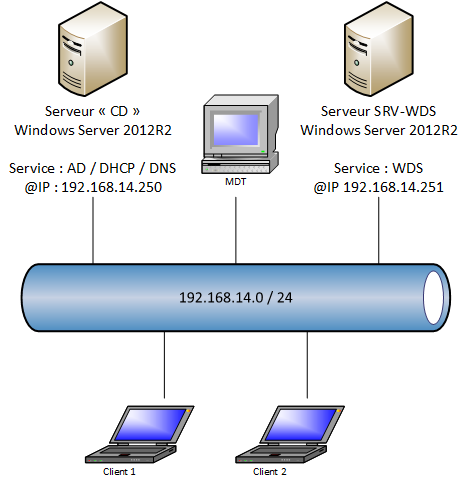
\includegraphics[scale=1.2]{Pictures/Plan.png}
\end{figure}
\newpage

% ##### Page 4 #####
\section{Avant de commencer}
Avant de mettre en production, il était nécessaire de réaliser un plan de déploiement sur des machines virtuelles ainsi que les différentes tâches à faire.

\subsection{Tâches à faire}
\subsubsection{Configuration à faire}
\begin{itemize}
\item Faire un \textbf{contrôleur de domaine}.
\item Héberger le domaine \textbf{cliniques-ouest.fr} sur le contrôleur de domaine.
\item Mettre les \textbf{services DHCP et DNS (si besoin)} sur le contrôleur de domaine.
\item Intégrer les postes clients au domaine.
\item Mettre le \textbf{service WDS} et \textbf{ses fonctionnalités} sur un serveur nommé \textbf{SRV-WDS}
\end{itemize}

\subsection{Matériel à disposition}
\subsubsection{Matériel Physique}
\begin{itemize}
\item Windows Server 2012R2
\item Processeur Intel Core 2 Duo E8500 2C/2T
\item 8 Go de RAM.
\item Réseau Filaire 10/100/1000
\item Windows Server 2012R2
\item VmWare
\end{itemize}

\subsubsection{Matériel Virtuel}
\begin{itemize}
\item Windows Server 2012R2 pour le DC et SRV-WDS.
\item Machine Virtuelle sans OS pour faire \textbf{du BOOT PXE}.
\item Réseau privé géré par WmWare.
\end{itemize}
\newpage

% ##### Page 5 #####
\section{WDS}
\subsection{Installation du service}
Le serveur de déploiement Windows est accessible depuis le gestionnaire de serveur puis dans "Ajouter des rôles et fonctionnalités". Il faudra choisir "Services de déploiement Windows".\\
\begin{figure}[hbtp]
\centering
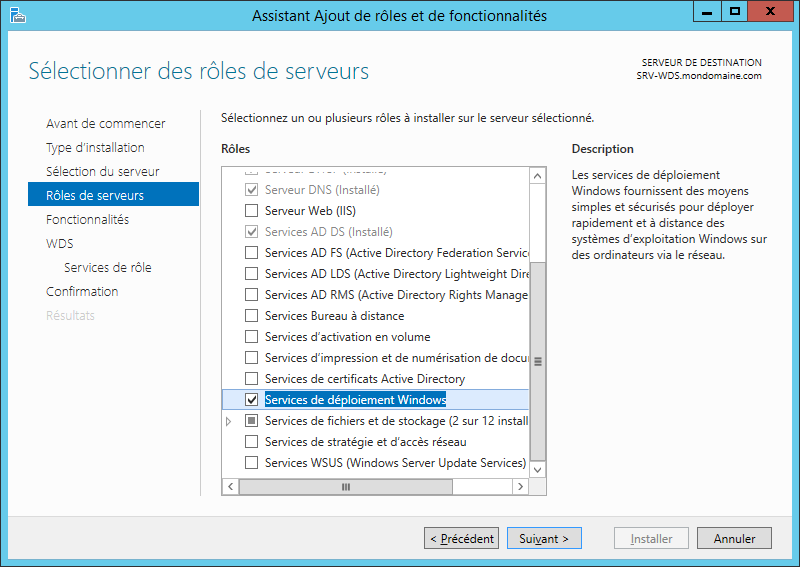
\includegraphics[scale=0.7]{Pictures/Installation/InstallWDS.png}
\caption{\label{etiquette} Rôles et fonctionnalités}
\end{figure}

L'écran de fonctionnalités ne sert à rien car la fonctionnalité voulue est déjà cocher donc il faut le passer cet écran en cliquant sur "Suivant"
\newpage

% ##### Page 6 #####
Il y a pas besoin de s'occuper de l'écran suivant car si on décoche ce qui a été cocher par le 1\ier{} écran, cela veut dire qu'on veut pas le faire.
\begin{figure}[hbtp]
\centering
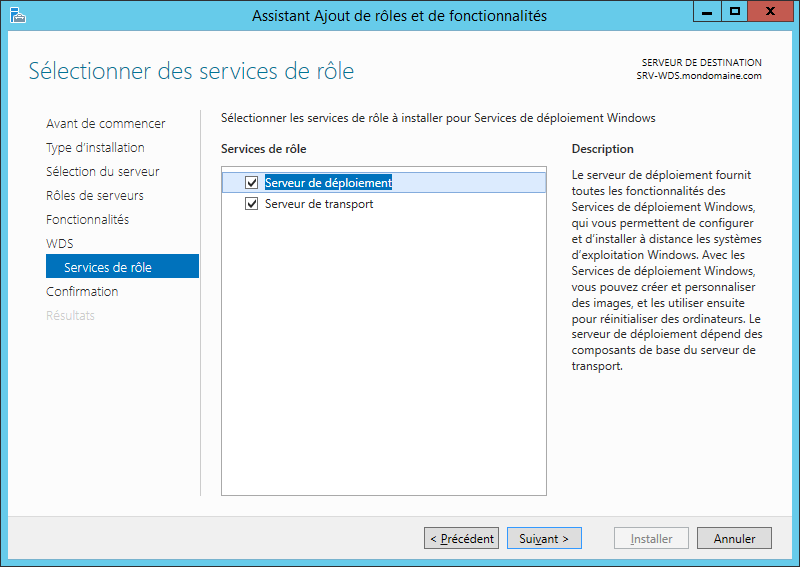
\includegraphics[scale=0.7]{Pictures/Installation/InstallRole.png}
\caption{\label{etiquette} Services de rôle}
\end{figure}

Le processus d'installation est rapide et un redémarrage n'est pas nécessaire. Suite à cette installation, il reste à faire le paramétrage.

\begin{figure}[hbtp]
\centering
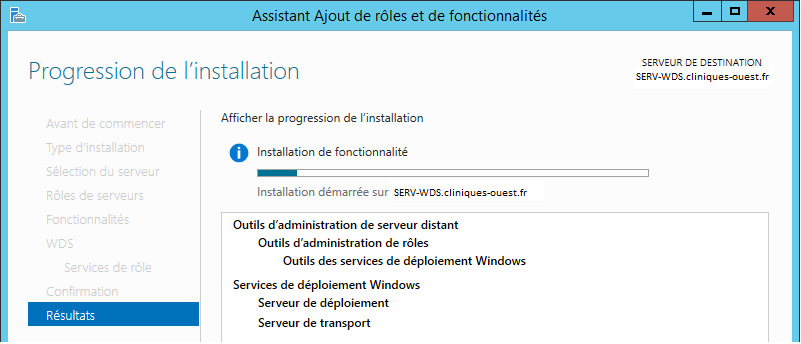
\includegraphics[scale=0.7]{Pictures/Installation/InstallWDS4.png}
\caption{\label{etiquette} Services de rôle}
\end{figure}
\newpage

% ##### Page 7 #####
\subsection{Configuration de WDS}

Notre service de déploiement fraîchement installé, nous allons premièrement devoir configurer le serveur en faisant un \textbf{clique droit} sur le serveur puis \textbf{Configurer le serveur}\\

Notre serveur de déploiement s'appelle donc \textbf{SERV-WDS.cliniques-ouest.fr}

\begin{figure}[hbtp]
\centering
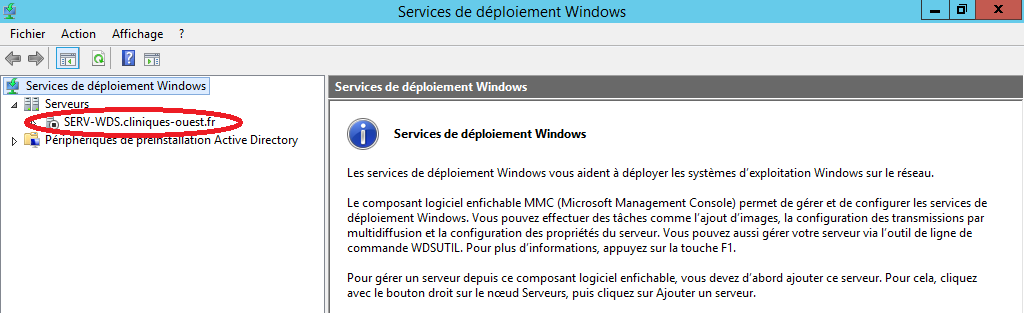
\includegraphics[scale=0.68]{Pictures/Configuration/Conf1.png}
\caption{\label{etiquette} 1ère configuration}
\end{figure}

Suite à cela, toute une configuration pas-à-pas est à faire pour faire le configuration du serveur en prenant en compte les 4 points suivants.

\begin{figure}[hbtp]
\centering
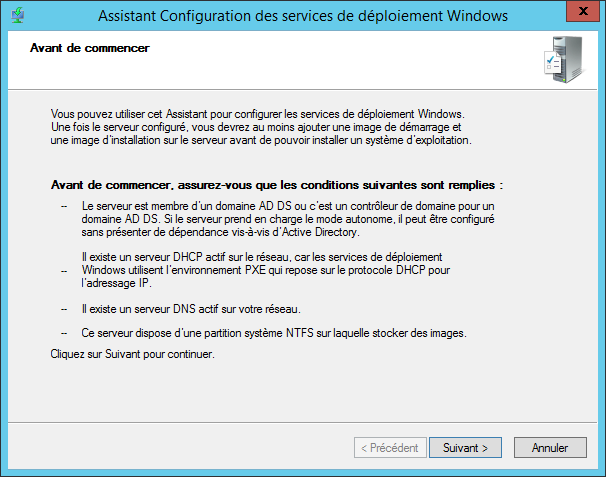
\includegraphics[scale=0.82]{Pictures/Configuration/Conf2.png}
\caption{\label{etiquette} Assistant Configuration}
\end{figure}
\newpage

% ##### Page 8 #####
Dans notre cas, ce serveur de déploiement est intégré à un domaine avec un service DHCP / DNS sur le DC et en plus, nous avons mis un second disque dur à la machine virtuelle pour y stocker les images de déploiement qu'il faut renseigner ici : \textbf{\path{E:\WDS\Deploy}} \\

\begin{figure}[hbtp]
\centering
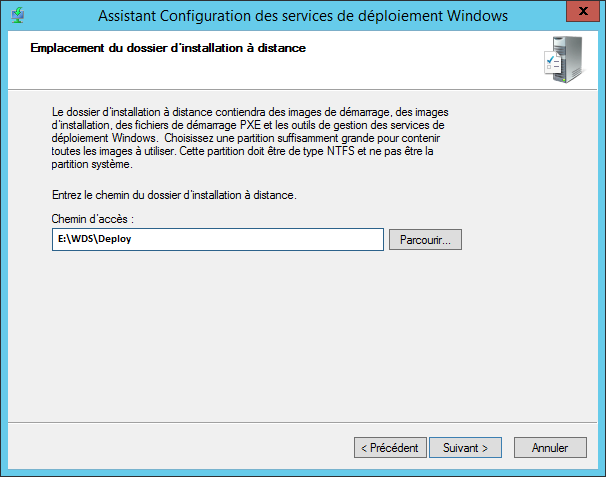
\includegraphics[scale=0.8]{Pictures/Configuration/Conf4.png}
\caption{\label{etiquette} Emplacement Image d'installation}
\end{figure}

Le dossier d’installation contient les images de démarrage, images d’installation, fichier de démarrage PXE, et les outils de gestion des services de déploiement Windows. \\

L'étape suivante consiste à configurer le service DHCP mais le nôtre n'est pas sur SERV-WDS mais sur le DC donc il faudra configurer manuellement les options DHCP sur le DC . Il faut donc laisser les options par défaut

\begin{figure}[hbtp]
\centering
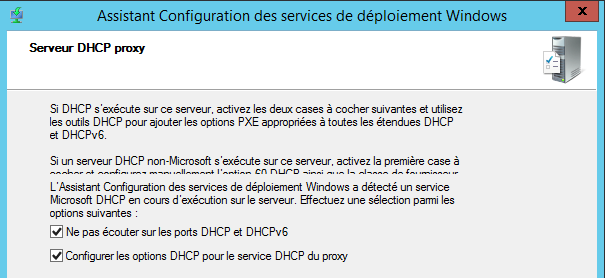
\includegraphics[scale=0.8]{Pictures/Configuration/Conf5.png}
\caption{\label{etiquette} Option DHCP}
\end{figure}

\newpage

% ##### Page 9 #####

Cocher ensuite "Répondre à tous les ordinateurs clients ..." Puis "Suivant" pour que les ordinateurs puissent être déployer qu'il soit ou non dans l'Active Directory (pour les nouveux postes)

\begin{figure}[hbtp]
\centering
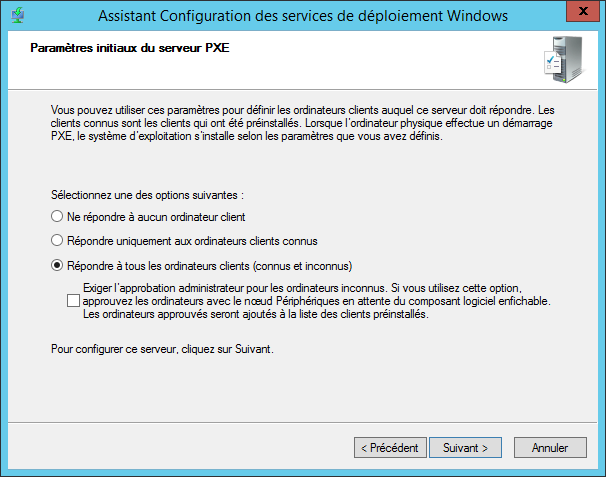
\includegraphics[scale=0.7]{Pictures/Configuration/Conf6.png}
\caption{\label{etiquette} Option PXE}
\end{figure}

Il nous reste à démarrer le serveur avec un clique droit puis "Toutes les tâches" --> "Démarrer".

\begin{figure}[hbtp]
\centering
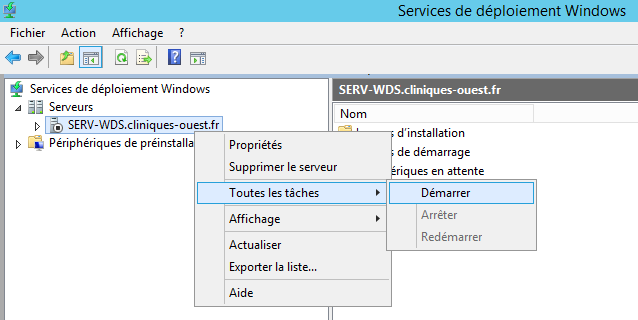
\includegraphics[scale=0.7]{Pictures/Configuration/Conf7.png}
\caption{\label{etiquette} Démarrage du service}
\end{figure}
\newpage

% ##### Page 10 #####
\subsection{Ajout de l'image de démarrage Windows}
Pour réaliser un déploiement à distance deux fichiers au minimum sont nécessaires:

\begin{itemize}
\item Un premier fichier de démarrage qui permettra au poste distant de charger le système : \textbf{boot.wim}
\item  Puis un second fichier qui contiendra les sources d’installation : \textbf{install.wim} \\
\end{itemize}

Les 2 fichiers se trouvent sur le CD ou l'ISO de Windows mais depuis Windows 10, il existe un fichier \textbf{install.esd} qu'il faut convertir avec DISM. \\

Se rendre ensuite dans « Image de démarrage » et « Ajouter une image de démarrage... »
\begin{figure}[hbtp]
\centering
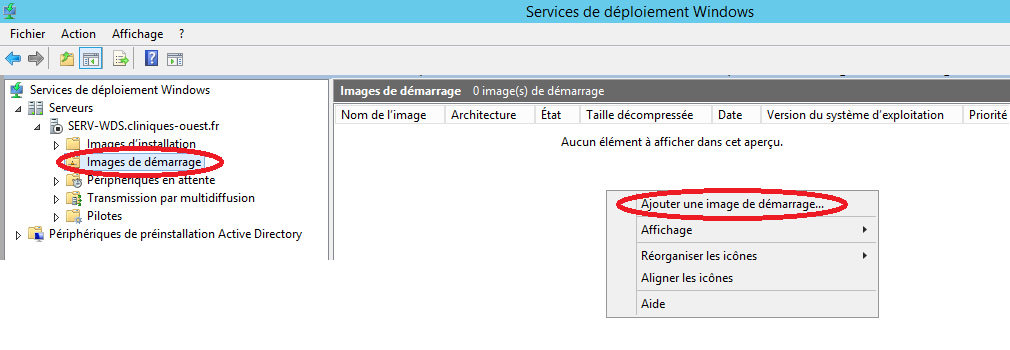
\includegraphics[scale=0.7]{Pictures/Configuration/Conf8.png}
\caption{\label{etiquette} Image de démarrage}
\end{figure}

Et à partir de là, on peut ajouter l'image Windows voulu en montant l'image ISO ou le disque en indiquant le chemin absolu du fichier \textbf{boot.wim} 

\begin{figure}[hbtp]
\centering
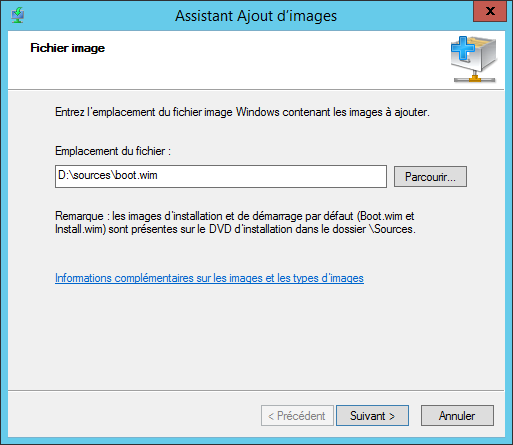
\includegraphics[scale=0.7]{Pictures/Configuration/Conf9.png}
\caption{\label{etiquette} Image de démarrage}
\end{figure}
\newpage

% ##### Page 11 #####
L'étape suivante permet de changer le nom d'affichage et la description affichée pendant le démarrage et ce sera la dernière à valider pour commencer à charger l'image sur le serveur WDS

\begin{figure}[hbtp]
\centering
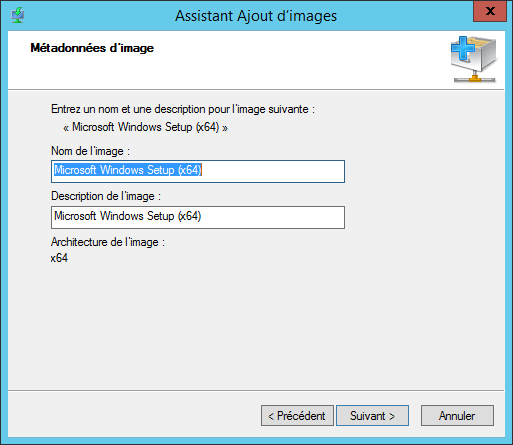
\includegraphics[scale=0.7]{Pictures/Configuration/Conf10.png}
\caption{\label{etiquette} Nom de l'image}
\end{figure}
\begin{figure}[hbtp]
\centering
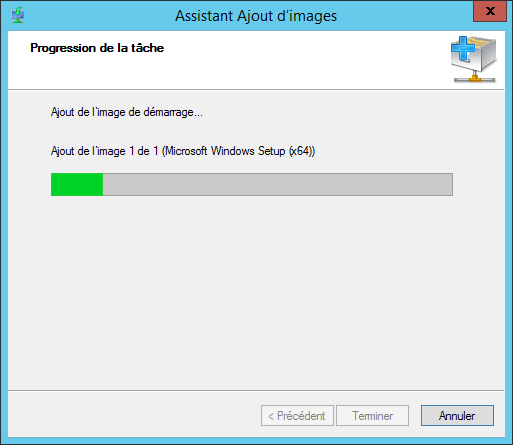
\includegraphics[scale=0.7]{Pictures/Configuration/Conf11.png}
\caption{\label{etiquette} Déploiement de l'image sur le serveur}
\end{figure}
\newpage

% ##### Page 12 #####
\subsection{Ajout de l'image d'installation Windows}

L'image d'installation contient TOUTES les éditions Windows preséntent dans le CD ou l'ISO. Cette étape va permettre de choisir l'édition de Windows pour être déployer. \\

Pour commencer, il faut aller dans le dossier « Images d’installation », faire un clic droit et choisir « Ajouter une image… ».

\begin{figure}[hbtp]
\centering
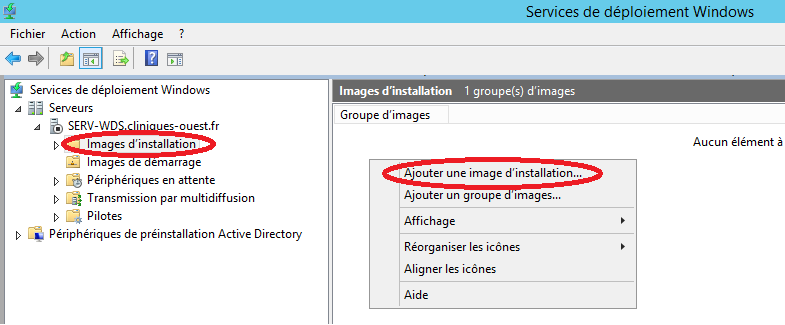
\includegraphics[scale=0.7]{Pictures/Configuration/Conf12.png}
\caption{\label{etiquette} Ajout de l'image d'installation}
\end{figure}

Un nom de groupe d’images va être demandé. On pourra alors donner un nom à un groupe d’image comme "Win8", "Win10", "serveur"...). Puis cliquer sur "Suivant".

\begin{figure}[hbtp]
\centering
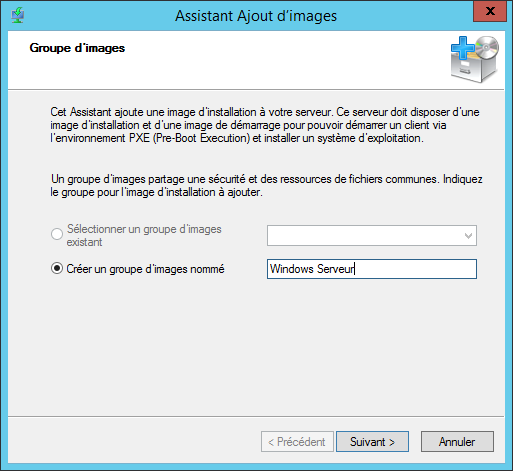
\includegraphics[scale=0.7]{Pictures/Configuration/Conf13.png}
\caption{\label{etiquette} Ajout de l'image d'installation}
\end{figure}
\newpage

% ##### Page 13 #####
Pour l’image, faite comme pour le précédent ficher en montant l'image ISO ou le disque en indiquant le chemin absolu du fichier \textbf{install.wim} et cliquer sur "Suivant"
\begin{figure}[hbtp]
\centering
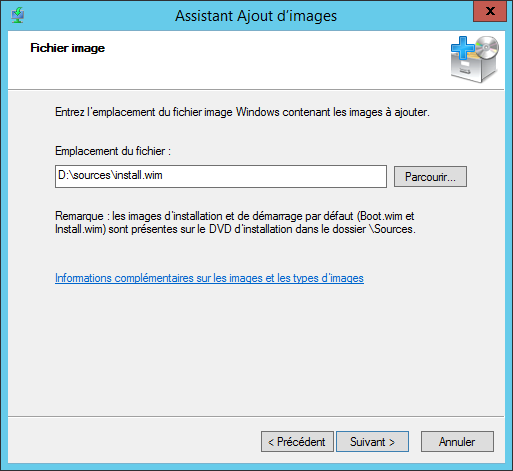
\includegraphics[scale=0.7]{Pictures/Configuration/Conf14.png}
\caption{\label{etiquette} Image d'installation}
\end{figure}

L'assistant va lire le fichier \textbf{install.vim} et on pourra choisir l'édition Windows voulue.
Dans notre cas, on va prendre l'édition \textbf{Windows 10 Professionnel}
\begin{figure}[hbtp]
\centering
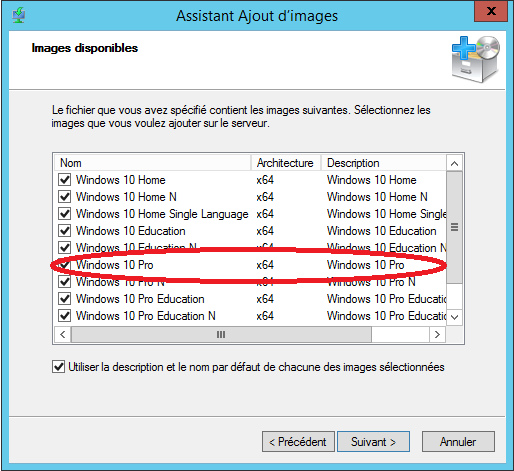
\includegraphics[scale=0.7]{Pictures/Configuration/Conf15.png}
\caption{\label{etiquette} Image d'installation}
\end{figure}
\newpage

% ##### Page 14 #####
L'étape suivante montre un résumé de notre choix d'image avant de procéder au chargement de cette dernière
\begin{figure}[hbtp]
\centering
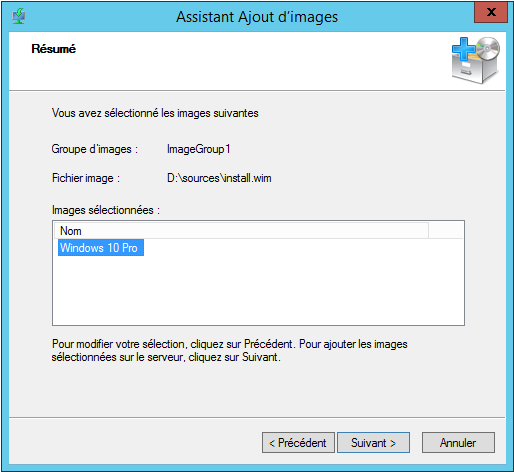
\includegraphics[scale=0.7]{Pictures/Configuration/Conf16.png}
\caption{\label{etiquette} Résumé}
\end{figure}

\subsection{Conclusion}

Le service WDS va servir à faire une installation de Windows via le BOOT PXE, cette méthode n'est pas entièrement automatique.\\

Pour faire un déploiement automatique de Windows, il faut utiliser en complément \textbf{Windows ADK} et \textbf{MDT}

% ################################################## CHARLY ######################################################

\newpage
% ##### Page 15 #####
\section{MDT}
\subsection{Installation du Kit Windows ADK}
 Le module \textbf{Microsoft Deployment Toolkit ou MDT}, se repose essentiellement sur le module WDS et \textbf{Windows Assessment and Deployment Kit (ADK)}. \\ \\
 Lors de l'installation de Windows ADK, choisir les options suivantes:
\begin{figure}[hbtp]
\centering
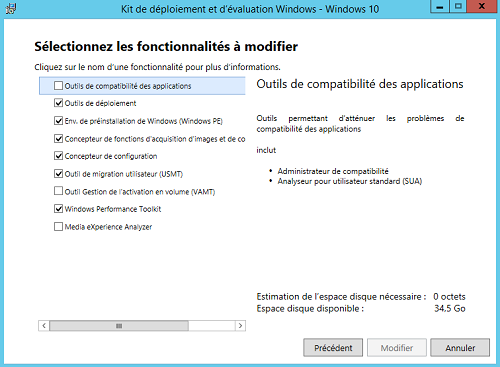
\includegraphics[scale=0.7]{Pictures/MDT/MDT1.png}
\caption{\label{etiquette} Fonctionnalités ADK}
\end{figure}

\subsection{Installation de la console MDT}
La console MDT nous permettra de mettre en place un déploiement d'image windows avec des fonctionnalités spécifiques.
\begin{figure}[hbtp]
\centering
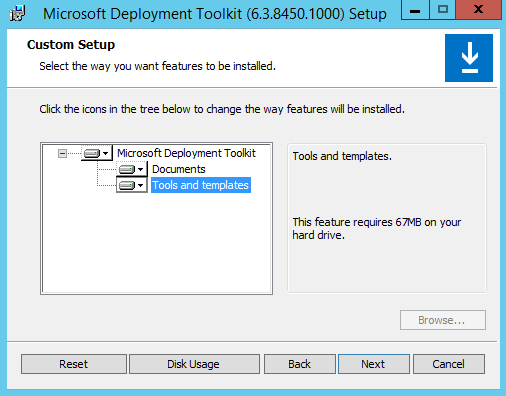
\includegraphics[scale=0.7]{Pictures/MDT/MDT2.png}
\caption{\label{etiquette} Fonctionnalités console MDT}
\end{figure}

\newpage
% ##### Page 15 #####
\subsection{Configuration de la Console MDT}
Un \textbf{« Deployment Share »} nous permettra de faire une image personnalisé de Windows. Pour configurer le tout, ouvrir l'application \textbf{"Deployment Workbench"}, faire un clic droit sur \textbf{« Deployment Share »} et choisir \textbf{« new deployment share »}
\begin{figure}[hbtp]
\centering
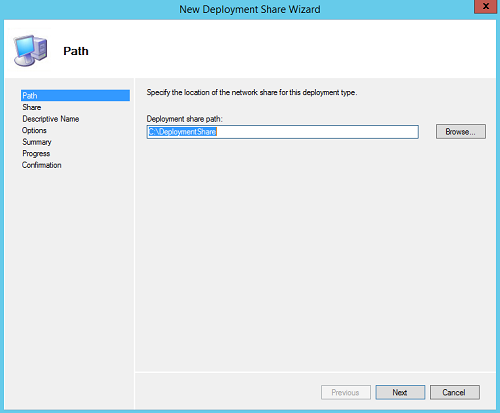
\includegraphics[scale=0.7]{Pictures/MDT/MDT3.png}
\caption{\label{etiquette} Configuration console MDT 1/3}
\end{figure}

Pendant cette installation, il vous sera demandé de mettre un nom au dossier \textbf{« Deployment Share »} qui sera partagé, de modifier le comportement de l'assistant de déploiement.
\begin{figure}[hbtp]
\centering
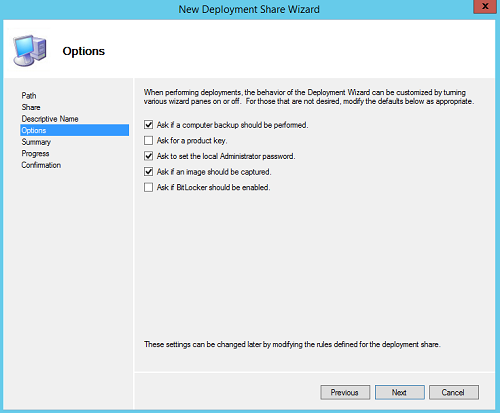
\includegraphics[scale=0.7]{Pictures/MDT/MDT4.png}
\caption{\label{etiquette} Configuration console MDT 2/3}
\end{figure}

\newpage
% ##### Page 16 #####
A la fin de l'installation, on obtiendra un affichage comme ceci. Voir ci-dessous.
\begin{figure}[hbtp]
\centering
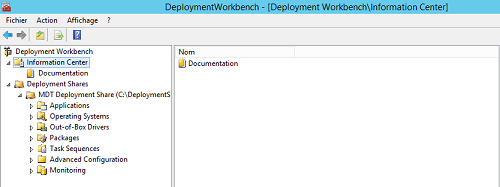
\includegraphics[scale=0.7]{Pictures/MDT/MDT5.png}
\caption{\label{etiquette} Configuration console MDT 3/3}
\end{figure}

Ce qui va nous intéresser dans un premier temps c'est \textbf{"Opérating System"}. Pour commencer, faites un clic droit sur le dossier "Opérating System" et il vous sera proposé d'ajouter une nouvelle image.\\
Lors de l'installation choisir \textbf{"full set of sources files"}, ensuite sélectionner votre CD / DVD. Enfin il vous proposera de mettre un nom à l'image.
\begin{figure}[hbtp]
\centering
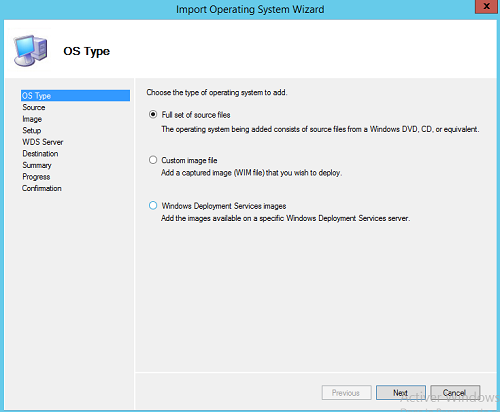
\includegraphics[scale=0.7]{Pictures/MDT/MDT6.png}
\caption{\label{etiquette} Operating System}
\end{figure}

\newpage
% ##### Page 17 #####
Le rôle de la séquence de tâche est d’exécuter une liste de tâches définies, qui s'effectuera lors de l'installation de l'OS avec les paramètres définis sur la tâche en question. Pour la création de cette tâche, faites un clic droit sur \textbf{"task sequence"}. Il vous sera demandé de mettre un numéro (ID) et le nom de votre organisation.
\begin{figure}[hbtp]
\centering
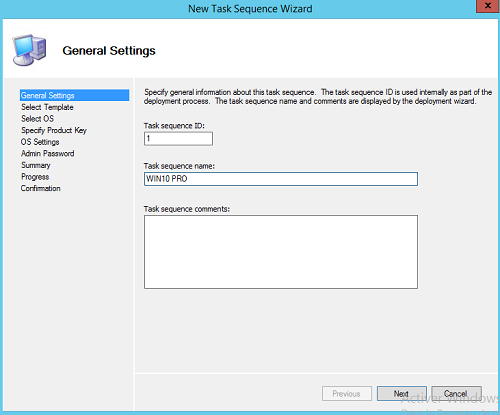
\includegraphics[scale=0.7]{Pictures/MDT/MDT7.png}
\caption{\label{etiquette} Task Sequence 1/2}
\end{figure}

Il vous sera aussi demandé de choisir l'OS, afin de lier celle-ci
\begin{figure}[hbtp]
\centering
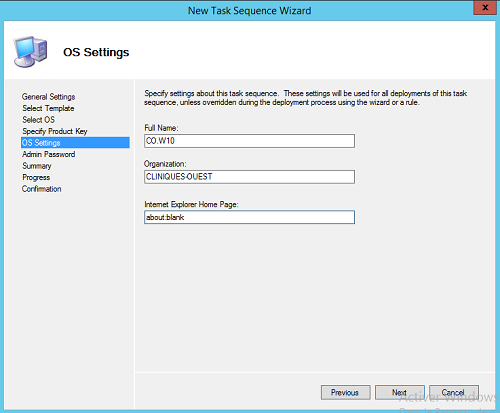
\includegraphics[scale=0.7]{Pictures/MDT/MDT8.png}
\caption{\label{etiquette} Task Sequence 2/2}
\end{figure}

\newpage
% ##### Page 18 #####
Le monitoring se situe dans les propriétés du dossier MDT situé dans le \textbf{"Deployment Workbench"}. L'option s'activera lorsque l'on aura coché la case [enable ...] située dans l'onglet monitoring des propriétés. Voir ci-dessous.
\begin{figure}[hbtp]
\centering
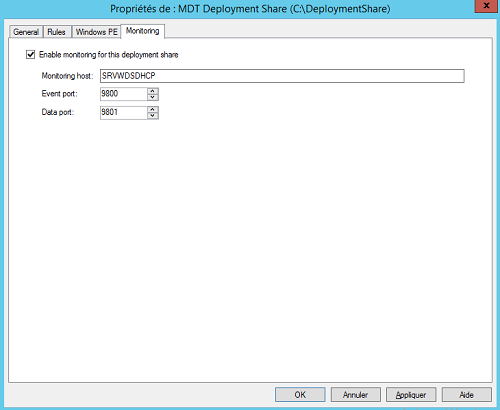
\includegraphics[scale=0.7]{Pictures/MDT/MDT9.png}
\caption{\label{etiquette} Réponses automatiser}
\end{figure}

Pour mettre à jour l'image, toujours sur le dossier MDT faite un clic droit, ensuite il vous est proposé \textbf{"Update Deployment Share Wizard"}.
Penser à bien mettre l'update en complète afin d'avoir une image propre.
\begin{figure}[hbtp]
\centering
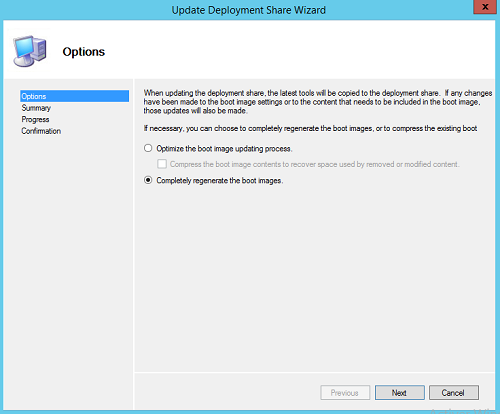
\includegraphics[scale=0.7]{Pictures/MDT/MDT10.png}
\caption{\label{etiquette} Mise à jour de l'image 1/2}
\end{figure}

\newpage
% ##### Page 19 #####
Pour vérifier que nos dernières modifications soient faite, les fichiers se trouve dans \textbf{"C:\textbackslash{}DeploymentShare puis dans boot"} suite à une nouvelle génération de l'image
\begin{figure}[hbtp]
\centering
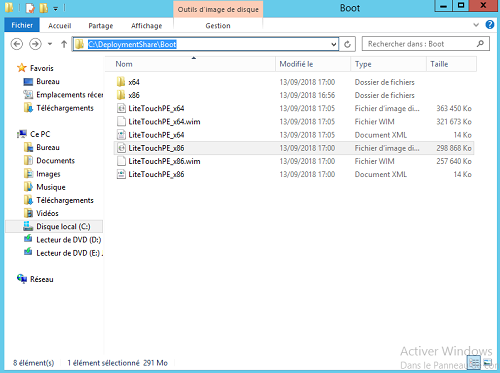
\includegraphics[scale=0.7]{Pictures/MDT/MDT11.png}
\caption{\label{etiquette} Mise à jour de l'image 2/2}
\end{figure}

Lorsque vous avez votre image en \textbf{LiteTouchPE x86"}, monter là sur votre VM. Une fois monter, mettre le fichier \textbf{"boot.wim"} dans le dossier images de démarrage se situant dans le service de déploiement windows.

\newpage
% ##### Page 20 #####
\subsection{Déploiement de l'image}
Lors d'un déploiement d'image Windows, appuyer sur F12 pour booter sur le réseau.
\begin{figure}[hbtp]
\centering
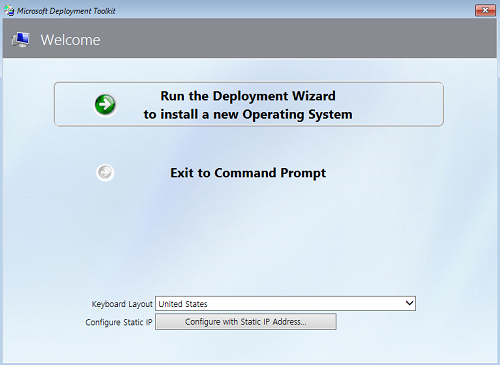
\includegraphics[scale=0.7]{Pictures/Deploiement/DEP1.png}
\caption{\label{etiquette} Déploiement 1/3}
\end{figure}

Il faudra choisir la tâche configurée auparavant.
\begin{figure}[hbtp]
\centering
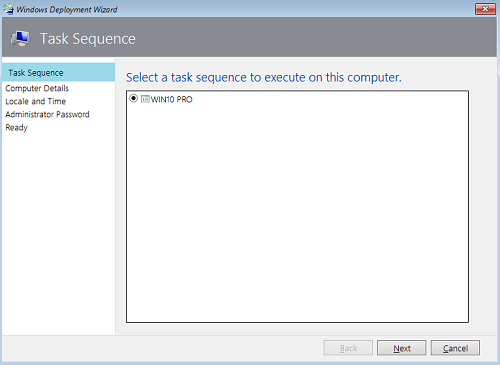
\includegraphics[scale=0.7]{Pictures/Deploiement/DEP2.png}
\caption{\label{etiquette} Déploiement 2/3}
\end{figure}

\newpage
Il vous sera demandé de mettre le mot de passe Administrateur.
\begin{figure}[hbtp]
\centering
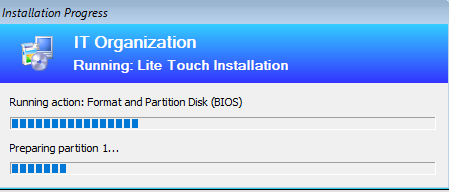
\includegraphics[scale=0.7]{Pictures/Deploiement/DEP3.png}
\caption{\label{etiquette} Déploiement 3/3}
\end{figure}
\subsection{Conclusion}
Comparé à WDS, la combinaison \textbf{Windows ADK} et \textbf{MDT} permet d'automatiser l'installation de Windows, ainsi que les pilotes, les pilotes, et même faire la fonction au domaine automatiquement.\\

MDT est un outil complèxe à utiliser et à configurer pour faire une automatisation totale de Windows.
\end{document}
